\section{Theoretical Justifications of AMP}

% \begin{frame}{Outline}
% \tableofcontents[currentsection]
% \end{frame}

\begin{frame}{AMP Finds Flatter Local Minima}

\begin{columns}
\column{0.72\textwidth}

We assume that the loss surface of each local minimum in $\mathcal{L}_\mathrm{ERM}$ can be {\em locally} approximated as an inverted Gaussian surface $\gamma$ with a mean vector $\boldsymbol{\mu}$ and a covariance matrix $\boldsymbol{\kappa}$.
\begin{theorem}[informal]
Under the locally Gaussian assumption, the empirical risk $\gamma(\boldsymbol{\theta};\boldsymbol{\mu},\boldsymbol{\kappa},A,C)$ is minimized when $\boldsymbol{\theta}=\boldsymbol{\mu}$ and the minimum value is $\gamma^\ast(\boldsymbol{\mu},\boldsymbol{\kappa},A,C)=C-A$. The minimum value of the AMP loss is the empirical risk at the location in the narrowest principal direction of the cross-section of the loss surface:
\begin{equation}
\gamma_\mathrm{AMP}^\ast(\boldsymbol{\mu},\boldsymbol{\kappa},A,C)=C-A\exp\left(-\frac{\epsilon^2}{2\sigma^2}\right)
\end{equation}
where $\sigma^2$ is the smallest eigenvalue of $\boldsymbol{\kappa}$.
\end{theorem}

% It is clear that $\gamma^\ast_\mathrm{AMP}$ although related to the minimum value of empirical risk $\gamma^\ast$, it also takes into account the curvature of the surface around the local minimum. Thus we can find a flatter minimum through minimizing $\mathcal{L}_\mathrm{AMP}$.

\column{0.28\textwidth}
\begin{figure}
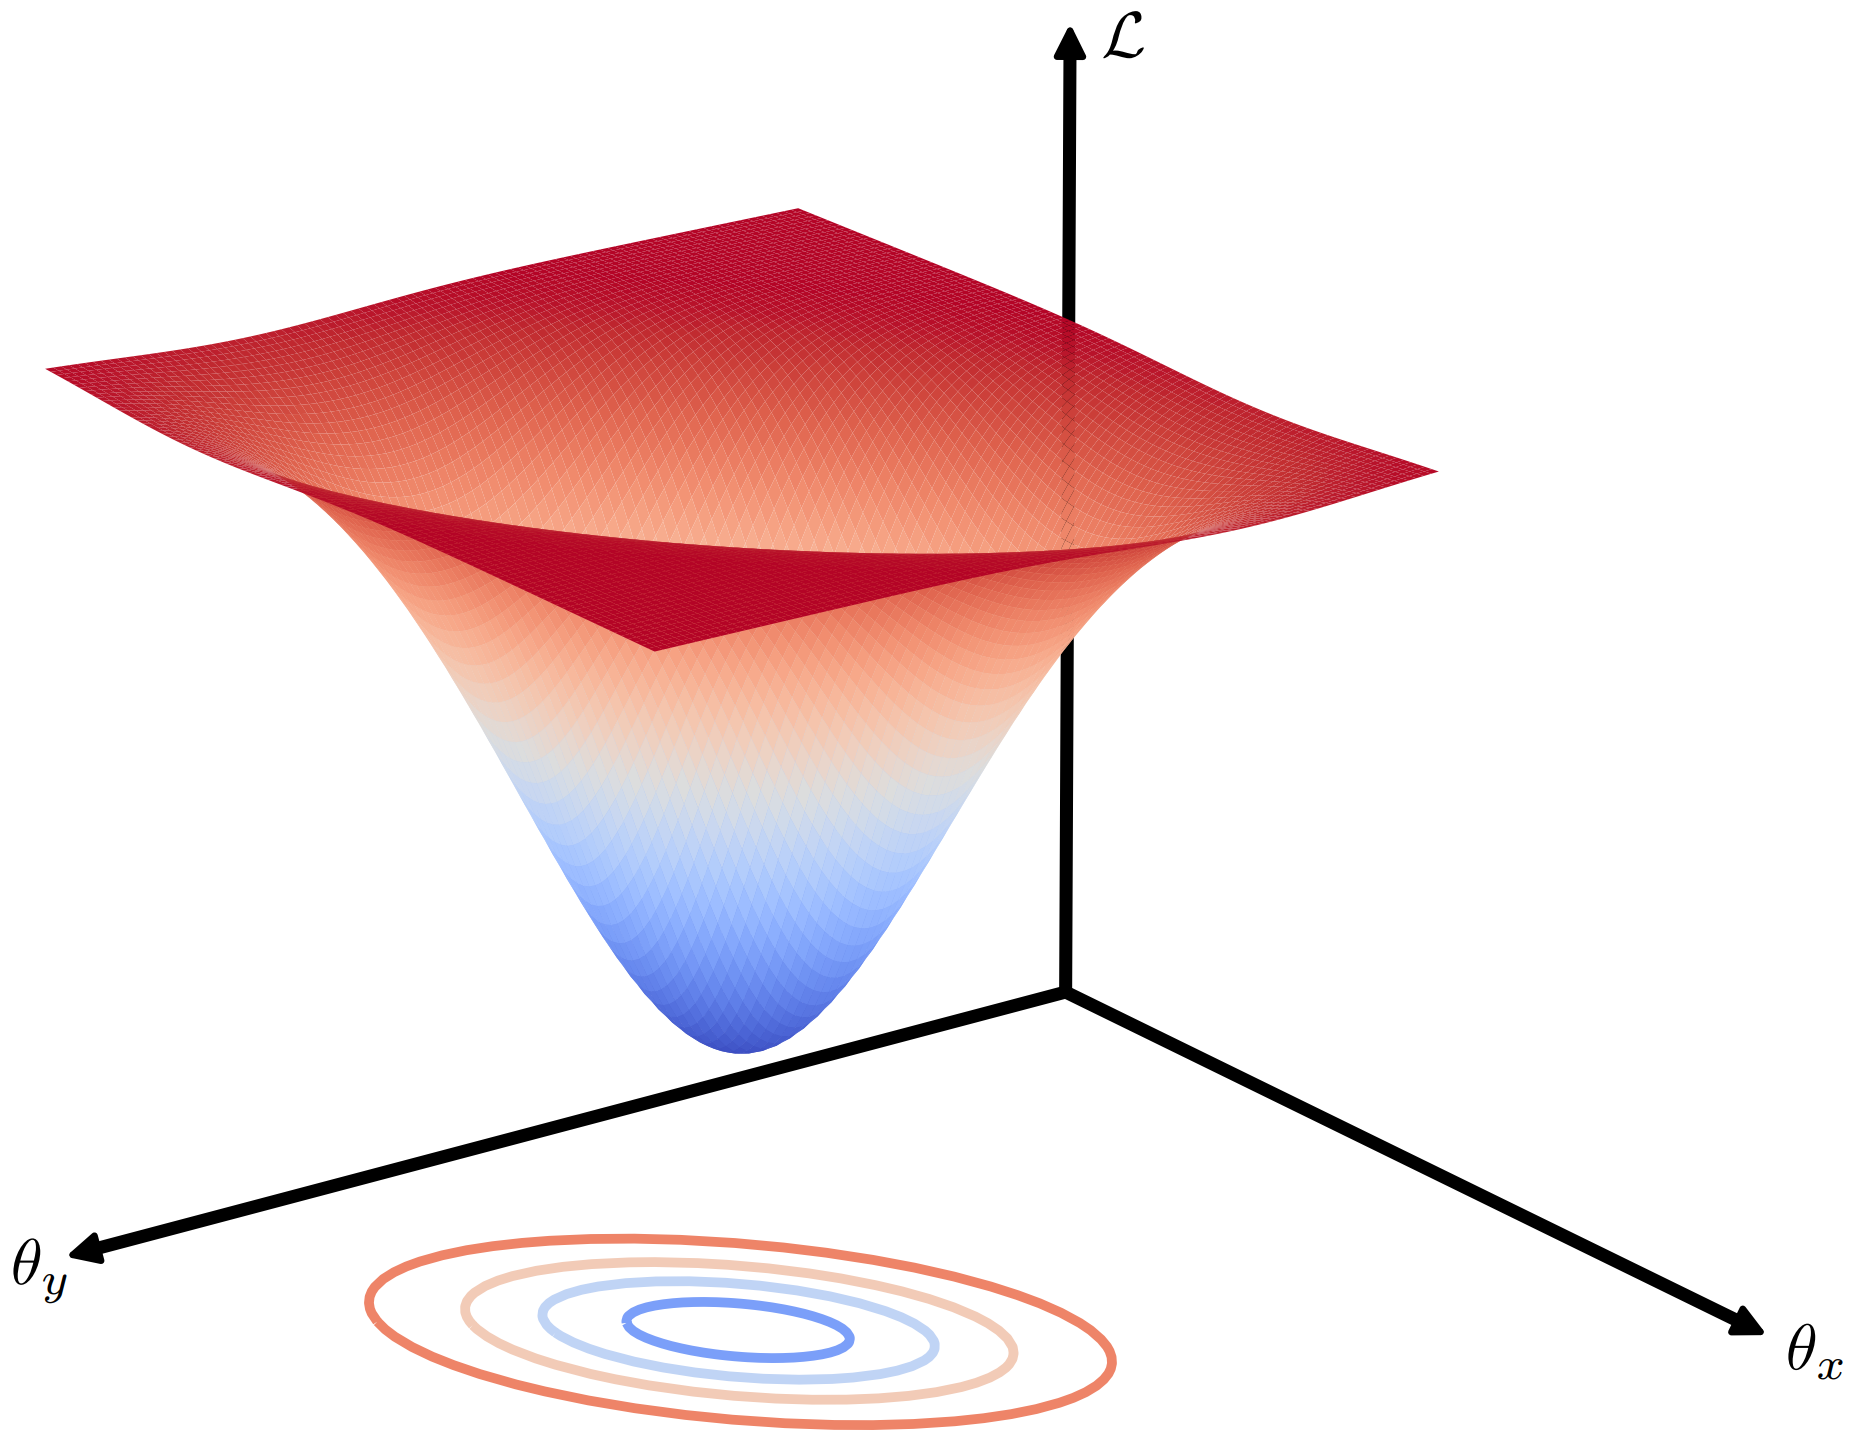
\includegraphics[width=.8\textwidth]{figs/surface.png}
\end{figure}
\begin{figure}
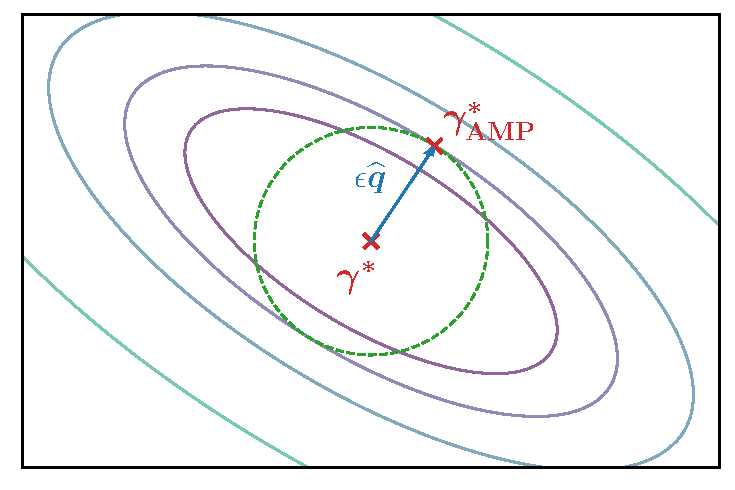
\includegraphics[width=.8\textwidth]{figs/gaussian.pdf}
\caption{The minimum values of $\gamma$ and $\gamma_\mathrm{AMP}$.}
\end{figure}
\end{columns}

\end{frame}

\begin{frame}{AMP Regularizes Gradient Norm}

\begin{theorem}[informal]
Consider that $N=1$, which is in fact used in our experiments. The AMP training is equivalent to ERM training with an additional term:
\begin{equation}
\widetilde{\mathcal{J}}_\mathrm{ERM}(\boldsymbol{\theta}):=\mathcal{J}_\mathrm{ERM}(\boldsymbol{\theta})+\Omega(\boldsymbol{\theta})
\end{equation}
where
\begin{equation}
\Omega(\boldsymbol{\theta}):=\begin{cases}
\zeta\Vert\nabla_{\boldsymbol{\theta}}\mathcal{J}_\mathrm{ERM}(\boldsymbol{\theta})\Vert_2^2,&\Vert\zeta\nabla_{\boldsymbol{\theta}}\mathcal{J}_\mathrm{ERM}(\boldsymbol{\theta})\Vert_2\le\epsilon\\
\epsilon\Vert\nabla_{\boldsymbol{\theta}}\mathcal{J}_\mathrm{ERM}(\boldsymbol{\theta})\Vert_2,&\Vert\zeta\nabla_{\boldsymbol{\theta}}\mathcal{J}_\mathrm{ERM}(\boldsymbol{\theta})\Vert_2>\epsilon
\end{cases}
\end{equation}
\end{theorem}

% Thus, the AMP training algorithm effectively tries to find the local minima of empirical risk that not only have low values, but also have small gradient norm near the minima. Note that a minimum with smaller gradient norms around it is a flatter minimum.

\end{frame}
